%%%%%%%%%%%%%%%%%%%%%%%%%%%%%%%%%%%%%%%%%%%%%%%%%%%%%%%%%%%%%%%%%%%%%%%%%%%

\documentclass{standalone}

\usepackage{amsmath}
\usepackage{mathptmx}
\usepackage{pgfplots}
\usetikzlibrary{external}
\tikzexternalize{copper-decay-linear}
\pgfplotsset{compat=1.16}

%% IEEE uses Times Roman font, so we'll default to Times.
%% These three commands make up the entire times.sty package.
\renewcommand{\rmdefault}{ptm}
\renewcommand{\ttdefault}{pcr}
\normalfont\selectfont

\begin{document}

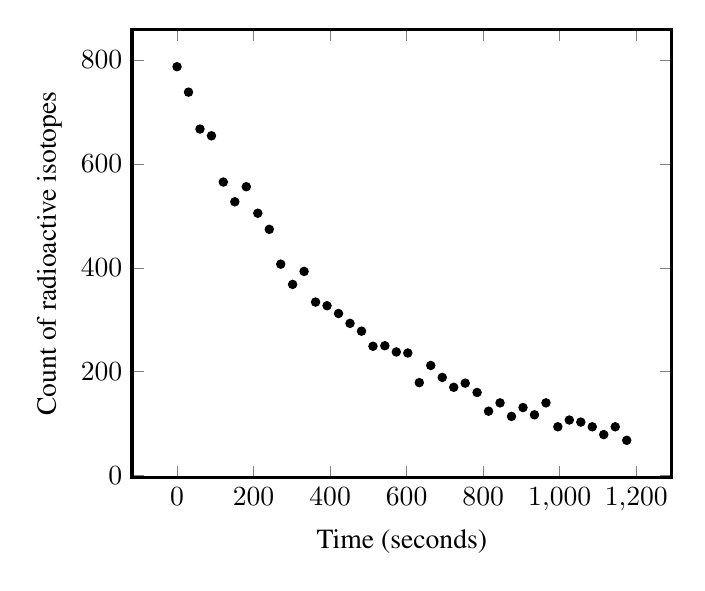
\begin{tikzpicture}
\tikzset{%%
  every mark/.append style={scale=1.0},%%
  scale=1.0%%
}
\pgfplotsset{%%
  every axis/.append style={font=\normalsize}%%
}
%%
\begin{axis}[%%
  axis line style=very thick,%%
  dotStyle/.style={mark size=1.5,black,mark color=black,mark=*,only marks},%%
  enlargelimits=true,%%
  %% x axis
  xlabel={\normalsize Time~(seconds)},%%
  %% y axis
  ylabel={\normalsize Count of radioactive isotopes}%%
]
%%
%%
\addplot[dotStyle] coordinates {
  (0, 787)
  (30, 738)
  (60, 667)
  (90, 654)
  (121, 565)
  (151, 527)
  (181, 556)
  (211, 505)
  (241, 474)
  (271, 407)
  (302, 368)
  (332, 393)
  (362, 334)
  (392, 327)
  (422, 312)
  (452, 293)
  (482, 278)
  (512, 249)
  (543, 250)
  (573, 238)
  (603, 236)
  (633, 179)
  (663, 212)
  (693, 189)
  (723, 170)
  (753, 178)
  (784, 160)
  (814, 124)
  (844, 140)
  (874, 114)
  (904, 131)
  (934, 117)
  (964, 140)
  (995, 94)
  (1025, 107)
  (1055, 103)
  (1085, 94)
  (1115, 79)
  (1145, 94)
  (1175, 68)
};
\end{axis}
\end{tikzpicture}

\end{document}
